\documentclass[12pt]{article} %tamaño mínimo de letra 11pto.

\usepackage{siunitx}
\usepackage{caption}
\usepackage{subcaption}
\usepackage{cite}
\usepackage{graphicx} 
\usepackage[english]{babel} %Español 
\usepackage[utf8]{inputenc} %Para poder poner tildes
\usepackage{vmargin} %Para modificar los márgenes
\setmargins{2.5cm}{1.5cm}{16.5cm}{23.42cm}{10pt}{1cm}{0pt}{2cm}
%margen izquierdo, superior, anchura del texto, altura del texto, altura de los encabezados, espacio entre el texto y los encabezados, altura del pie de página, espacio entre el texto y el pie de página
\usepackage{booktabs}
\usepackage{multirow}
\usepackage[table,xcdraw]{xcolor} 
\usepackage{multicol}



\begin{document}
%%%%%%Portada%%%%%%%
\begin{titlepage}
\centering
{ \bfseries \Large UNIVERSIDAD COMPLUTENSE DE MADRID}
\vspace{0.5cm}

{\bfseries  \Large FACULTAD DE CIENCIAS FÍSICAS} 
\vspace{1cm}

{\large DEPARTAMENTO DE ESTRUCTURA DE LA MATERIA, FÍSICA TÉRMICA Y ELECTRÓNICA}
\vspace{0.8cm}

%%%%Logo Complutense%%%%%
{
\includegraphics[width=0.35\textwidth]{figuras/logoUCM.png}} %Para ajustar la portada a una sola página se puede reducir el tamaño del logo
\vspace{0.8cm}

{\bfseries \Large TRABAJO DE FIN DE GRADO}
\vspace{15mm}

{\Large Código de TFG:  ETE20 } \vspace{5mm}

{\Large Imagen por Ultrasonidos}\vspace{5mm}

{\Large Ultrasound Imaging}\vspace{5mm}

{\Large Supervisor/es: Joaquín López Herraiz}\vspace{18mm} 

{\bfseries \LARGE Ignacio Ortega Alonso}\vspace{5mm} 

{\large Grado en Física}\vspace{5mm} 

{\large Curso acad\'emico 2020-2021}\vspace{5mm} 

{\large Convocatoria de junio}\vspace{5mm} 

\end{titlepage}
\newpage

{\bfseries \large Ultrasound imaging: B-line detection in lung ultrasound }\vspace{10mm} 

{\bfseries \large Abstract: }\vspace{5mm} 

Ultrasound imaging is a widely used technique for medical diagnosis. It is based on the emission of high-frequency sound waves and the detection of their returning echoes. Measuring time delays and changes in pressure amplitude of the received waves, the scanned object's structure and acoustical properties can be inferred. Despite their acoustical properties being unsuited for ultrasound imaging, lungs can also be examined with this technique. Certain artifacts known as B-lines which may appear in lung ultrasound are characteristic of pneumonia and similar pathologies such as COVID-19. Therefore, it has now become relevant to find methods able of detecting these artifacts. In this work, using a collection of assessed lung scans a machine learning classifier algorithm was trained to detect B-lines following two different approaches. One of them involves extracting specific features from the images that are representative of B-lines, while the other takes as an input the whole image to be classified. The second approach showed better results, while the results of the first one could be improved with changes in the extracted features and better quality data.
 
\vspace{1cm}

{\bfseries \large Resumen: }\vspace{5mm} 

La imagen por ultrasonidos es una técnica ampliamente utilizada para el diagnóstico médico. Se basa en la emisión de ondas de sonido de alta frecuencia y la posterior detección de sus ecos. Midiendo los tiempos de retardo y los cambios en la amplitud de presión de las ondas recibidas, se pueden deducir la estructura y las propiedades acústicas del objeto escaneado. A pesar de tener unas propiedades acústicas inadecuadas para la imagen por ultrasonidos, los pulmones también pueden ser examinados mediante esta técnica. Determinados artefactos conocidos como 'líneas B' que se pueden observar en la ecografía pulmonar son indicativos de neumonía y patologías similares como COVID-19. Por lo tanto, es ahora relevante encontrar métodos capaces de detectar estos artefactos. En este trabajo, utilizando una colección de exploraciones de pulmón evaluadas, un algoritmo clasificador de aprendizaje automático ha sido entrenado para detectar líneas B siguiendo dos enfoques diferentes. Uno de ellos involucra la extracción de rasgos específicos de las imágenes que sean representativos de las líneas B, mientras que el otro toma como entrada la imagen completa. El segundo enfoque demostrado mejores resultados, mientras que los resultados del primero podrían ser mejorados con cambios en los rasgos seleccionados y datos de mejor calidad.

\newpage


% CONTENTS 

\tableofcontents
\newpage

% ISSUES
%\begin{itemize}
%\color{red}
%\item dispersion relation: phase velocity / group velocity
%\item kind of transducer used
%\end{itemize}

% INTRODUCTION
\normalsize

\section{Introduction}

\subsection{Motivation and context}

\subsubsection{Medical Physics and Artificial Intelligence}
	
	% Medical Physics
	Medical Physics consists on the application of physical concepts to medicine. Among them we can find all the medical imaging techniques that are carried out in radiology units of hospitals for diagnosis, prognosis and follow-up of diseases, such as X-rays, computed tomography (CT), magnetic resonance imaging (MRI) or ultrasound (US), as well as positron emission tomography (PET), which belongs to the area of nuclear medicine. Furthermore, there are therapeutical applications too such as radiotherapy, which allows to treat tumors with the aid of ionizing radiation.
	
	% Artificial Intelligence
	Artificial Intelligence (AI) is an umbrella term that englobes many different models and algorithms designed to solve certain problems. In recent years, AI and in particular deep learning - a subcategory of the earlier - have shown great performance in several areas, medical physics being one of them \cite{shen}. For instance, it has been possible to detect skin cancer \cite{esteva} and pneumonia from chest X-rays \cite{rajpurkar} with great accuracy thanks to AI. There is such an interest in these techniques that the number of published articles on these topics in medical physics journals has grown exponentially (see fig. \ref{papers}).
	
	
\begin{figure}[h]
\centering
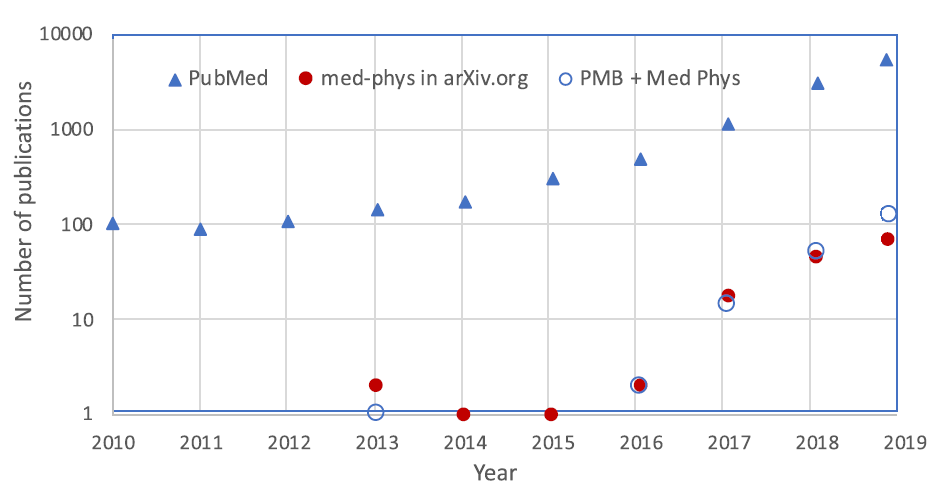
\includegraphics[width=0.6\textwidth]{figuras/DL_papers.png}	
\caption{\small The number of published papers on IA y DL has grown exponentially in recent years. \cite{shen}}
\label{papers}
\end{figure}
	
\subsubsection{Lung ultrasound and COVID-19}
	% Relevance of LUS in the Covid-19 pandemic context
	Recently, lung ultrasound (LUS) has become increasingly relevant due to the current situation of the COVID-19 pandemic. Despite CT being the most established imaging technique for pneumonia monitoring and assessment, lung ultrasound advantages make it a promising tool to face this health crisis. First, ultrasound does not use ionizing radiation, which makes it a suitable technique for pregnant women and children. In addition, it can be used in emergency and intensive care units without the need to take patients to the radiology unit, thus reducing the risk of infection and the workload for healthcare workers \cite{allinovi}. Lastly, diagnosis of Covid-19 with lung ultrasound has been proven to be comparable in accuracy to the CT standard \cite{ottaviani}.
	

	% Applications of AI to LUS
	Similarly to other fields of medical physics, lung ultrasound also has the potential of being improved by the use of AI. In lung ultrasound in particular it is of great importance to correctly identify certain artifacts known as B-lines (see section 1.2.4), whose presence is linked to different diseases, Covid-19 being one of them. An algorithm able to detect such artifacts would have multiple advantages: it would aid in the training of less experienced physicians, it could assist doctors in the diagnosis and it would speed up patient inspection times. Several of this type of algorithms have already been accomplished, both with the help of neural network classifiers \cite{vanSloun}\cite{born2020pocovid}\cite{cristiana2020automated}\cite{roy2020deep} and with more traditional algorithmic approaches \cite{brattain}\cite{moshavegh}.
	
	
\subsection{Physics of ultrasound imaging}
\subsubsection{Physical principles of ultrasound imaging}

	%(Overview)

	Medical ultrasound allows to obtain images of different body tissues thanks to the controlled emission of high-frequency sound waves (typically in the 1-10 MHz range) and the reception of their reflections. Ultrasound probes are equipped with piezoelectric transducers that vibrate when excited with high-voltage electric pulses. This vibration is then transmitted through the body as a pressure wave whose behaviour is influenced by the mechanical properties of the tissues. A fraction of the energy emitted by the probe is reflected on tissue interfaces and received by the transducers. The transducers then vibrate and produce an electric signal that is processed in order to create an image of the examined region. 
	
	%(Sound as a wave)
	
	Sound waves can be understood as periodic variations of pressure on a propagation medium. The rate at which the pressure varies (frequency $f$) and the spatial distance between neighbouring points with equal pressure (wavelength $\lambda$) are related through the speed of sound $c = \lambda f$. The speed of sound $c$ depends on the elastic properties of the propagation medium, and it can be expressed as a function of bulk modulus $B$ and density $\rho$ by:
	
\begin{equation}
c = \sqrt{ \frac{B}{\rho} }
\end{equation}
	
	In soft tissue, sound travels at an average speed of $ 1540 \si{\meter\per\second} $, but it can be as slow as $ 600 \si{\meter\per\second} $ in the lungs, or as fast as $ 3200 \si{\meter\per\second} $ in bones (see table \ref{tissues}). 
	
	%(Reflection and acoustic impedance)
	
	Another important property of a medium is acoustic impedance, which is defined as the product of the medium's density and speed of sound: 	

\begin{equation}
Z = \rho c
\end{equation}

	Differences in acoustic impedances of adjacent tissues are responsible for the reflection of sound waves. More exactly, the ratio between the pressure amplitudes of the reflected ($P_r$) and incident ($P_i$) wave can be expressed as	
	
\begin{equation}
\frac{P_r}{P_i} = \frac{Z_2 – Z_1}{Z_2 + Z_1}
\end{equation}
	
	where $Z_1, Z_2$ are the acoustic impedances of the proximal and distal tissues respectively. An intensity reflection coefficient can also be defined as: 	
	
\begin{equation}
R_I = \frac{I_r}{I_i} = \left( \frac{P_r}{P_i} \right)^2
\end{equation}
	
	making use of the fact that intensity is proportional to the squared power of pressure amplitude. For some interfaces such as fat-muscle this coefficient is very small, meaning that most of the energy carried by the wave keeps propagating. For others, such as muscle-air almost all the energy is reflected.

	%(Scattering)
	
	When the size of the objects responsible for reflection is similar or smaller than the wavelength, sound is reflected in all directions or scattered. The amount of scattered energy depends on acoustic impedance differences, but also on the texture of the tissue and the wavelength.

	%(Attenuation)
	
	Scattering, together with tissue absorption, are responsible for the attenuation or loss of energy of the propagating waves. Different tissues have different attenuation coefficients. They are typically measured in units of $dB/cm$ and are proportional to frequency. In other words, waves with larger wavelengths can penetrate deeper into the body. \cite{bushberg}

\begin{table}[]
\centering
\begin{tabular}{l|l|l|l|l}
            & $  \rho (kg  \cdot m^{-3})$ & $c (m \cdot s^{-1})$ & $Z (kg \cdot m^{-2} \cdot s^{-1})$ &  \\ \cline{1-4}
Air         & $1.2$                       & $330$                & $400$                              &  \\
Lung        & $300$                       & $600$                & $1.8 \cdot 10^5$                   &  \\
Fat         & $924$                       & $1450$                & $1.3 \cdot 10^6$                   &  \\
Soft tissue & $1050$                      & $1540$               & $1.6 \cdot 10^6$                   &  \\
Muscle      & $1068$                      & $1600$               & $1.7 \cdot 10^6$                   & \\
Bone        & $1650$                      & $3200$               & $5.3 \cdot 10^6$                   & 
\end{tabular}
\caption{\small Typical values of density, speed of sound and acoustical impedance for common tissues found in medical ultrasound. \cite{farr}}
\label{tissues}
\end{table}


\subsubsection{Transducers and beam properties}

	%(Transducers)

	Ultrasound waves are produced by transducers made of piezoelectric materials. Because of the way electric dipoles are arranged in this kind of materials, they vibrate when a voltage difference is applied to their surfaces. Similarly, when an external force makes them contract or expand, a difference in voltage appears between their surfaces. This property allows them to operate both as transmitters and receivers of sound waves. An important property of a transducer is its Q factor, which is defined as the ratio between its resonant frequency $f_0$ and the bandwith of the emitted pulse $ \Delta f$, that is, the range of frequencies around $f_0$ where energy is also emitted: 
	
\begin{equation}
Q = \frac{f_0}{\Delta f} 
\end{equation}

These frequencies are introduced by dampening the vibration of the piezoelectric and thus making the emitted pulse shorter. Transducers that are lightly damped show a  narrow bandwith (high Q factor) and a long spatial pulse length, whereas heavily damped transducers have broad bandwiths (low Q factor) and short spatial pulse length (figure \ref{pulse}). 

\begin{figure}[h]
\centering

\begin{subfigure}[b]{0.49\textwidth}
\centering
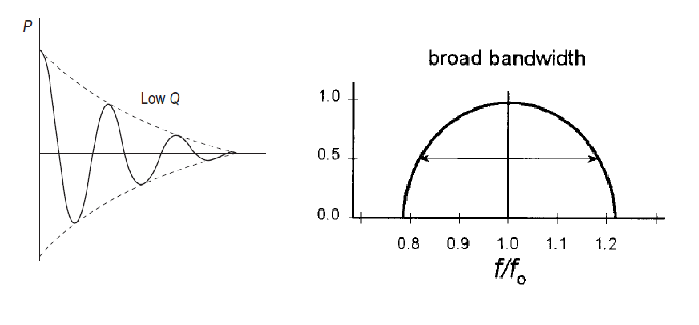
\includegraphics[width=\textwidth]{figuras/lowq.png}
\caption{\footnotesize A heavily damped transducer results in a short pulse and a  spectrum with broad bandwith.}
\end{subfigure}
\begin{subfigure}[b]{0.49\textwidth}
\centering
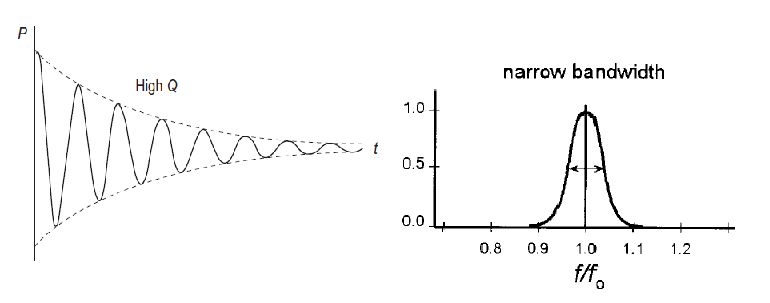
\includegraphics[width=\textwidth]{figuras/highq.png}
\caption{\footnotesize A lightly damped transducer results in a long pulse 				and a spectrum with narrow bandwith.}
\end{subfigure}	

\caption{\small Comparison of a low Q pulse (a) and high Q pulse (b): the amount of dampening of the transducer affects the length of the emitted pulse and consequently the bandwith of its spectrum. \cite{bushberg}\cite{farr}}
\label{pulse}	
\end{figure}

	%(Near and far field)
	
	Several piezoelectric elements are arranged in transducer arrays and operate together to produce an ultrasound beam. The shape of the beam is the result of interferences between every emitter. It is characterized by two regions: a near field where the beam converges and a far field where it diverges. The length of the near field $l$ (or in other words, the focal distance) is proportional to the square of the effective diameter of the transducer $d$ and inversely proportional to the emitted frequency $f$: 
	
\begin{equation}
l \propto \frac{d^2}{\lambda}
\end{equation}

That is, wider transducers and higher frequencies result in larger focal distances.

	%(Spatial resolution)
	
	The ability to resolve objects in the acquired image is determined by a series of parameters of the beam and transducers. In the axial direction (direction of the beam), resolution is limited by the spatial pulse length (SPL). Two returning echoes can only be resolved if the distance between them is greater than the SPL. Therefore, for two reflectors to be distinguished they cannot be separated by a distance shorter than half the SPL (fig. \ref{resolution}). Shorter SPL can be achieved with shorter wavelength or fewer cycles per pulse, i.e. lower Q factor. Typical axial resolution values are of $0.5 mm$. Because SPL is constant along the beam, axial resolution is independent of depth.
In the perpendicular direction resolution is determined by the diameter of the beam. For this reason lateral resolution is best at the focal zone and it decreases in the near and far fields. Some transducer arrays can produce beams of variable focal distance, creating an extended focal zone where lateral resolution is optimal. 

\begin{figure}
\centering
\begin{subfigure}[b]{0.4\textwidth}
\centering
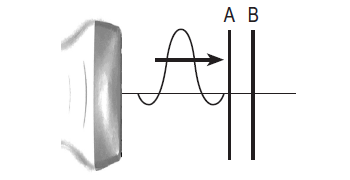
\includegraphics[width=\textwidth]{figuras/resolution1_edit.png}
\caption{\footnotesize A single pulse is emitted against interfaces A and B. The separation between the interfaces is $d$.}
\end{subfigure}
\centering
\hspace{3em}
\begin{subfigure}[b]{0.4\textwidth}
\centering
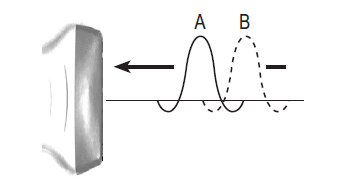
\includegraphics[width=\textwidth]{figuras/resolution2_edit.png}
\caption{\footnotesize Two pulses are reflected by interfaces A and B. The separation between the reflected pulses is $2d$.}
\end{subfigure}	
\caption{\small Spatial resolution along axial direction is determined by half the spatial pulse length ($SPL$). Two adyacent interfaces A and B separated by a distance $d$ can only be resolved if $d$ is greater than $\frac{1}{2} SPL$. \cite{farr}}
\label{resolution}
\end{figure}


\subsubsection{Image formation}
	
	In order to generate a two-dimensional ultrasound image several steps have to be followed. First transducers are set to 'transmit mode' to produce sound pulses using a high voltage spike. After the pulse is emitted, they are set to 'receive mode' in order to capture vibrations of returning echoes. Echoes received earlier correspond to reflections taking place close to the transducer, while later echoes are produced by deeper reflectors.  The returning echoes are very weak and can only induce small voltages in the transducers that need to be amplified. In addition, later echoes are significantly weaker than earlier ones due to attenuation experienced by the sound wave throughout its round-trip. To compensate for this an additional time-dependent amplification known as time gain compensation (TGC) is introduced. The outcome of this process is a signal containing information of the scanned tissues along the beam direction, where amplitude is proportional to acoustic impedance differences and time corresponds to depth. Assuming an average speed of sound of $c = 1540 m/s$ along the beam path, time $t$ and depth $D$ are related through: 
	
\begin{equation}
D = \frac{c·t}{2} 
\end{equation}

The $2$ factor accounts for the round-trip distance. After a certain time interval, transducers are set to emit the next pulse and the whole process is repeated several times per second with different focus parameters to achieve a two-dimensional image. 

\subsubsection{Lung Ultrasound and artifacts}

	%(Artifacts)

	As with any other imaging device, ultrasound cannot reproduce anatomy with unlimited accuracy. Artifacts are deviations from the actual aspect of the scanned objects due to the intrinsic working principles of the device. Lungs are particularly prone to exhibit artifacts when probed with ultrasound, but valuable information can still be obtained from its examination when the origin of these artifacts is well understood. 
	
	A typical lung ultrasound image shows the following features (see fig.\ref{artifacts}). First, a very bright and approximately horizontal line can be seen in the upper half of the picture, corresponding to the pleura. The pleura is a thin membrane inside the chest cavity where lungs are contained. The ribs can be also observed when the probe is perpendicular to them. They appear as dark regions above the pleura projecting shadows downwards. Due to the high difference of acoustic impedance between the soft tissue above the pleura and the air-filled lung below it, almost all the energy carried by sound waves is reflected, making observation of deeper tissues impossible. 
	
	A common artifact that can be observed in the region below the pleural line is A-lines (see fig.\ref{artifacts}-a). A-lines appear like equally distanced bright lines parallel to the pleural line and they can be explained as a reverberation artifact. Due to the high reflectivity of the pleura, echoes can bounce back and forth several times between it and the transducer surface. Because of their delay with respect to the emitted pulse, these echoes are interpreted as multiple objects located further away from the transducer \cite{artifacts}.

	%(B-lines)
	
	Another reverberation artifact that can be commonly observed in lung ultrasound is B-lines (see fig.\ref{artifacts}-c). Whereas A-lines are usually present in healthy lungs, B-lines are correlated with interstitial syndrome, a kind of disease where inflammation or acummulation of fluid makes thin tissues within the lung called interstitium to thicken and become denser. This can be observed for example in pneumonia patients. While the exact origin of this artifact is not clearly understood, it is thought that it is originated from reverberation between closely located high reflective surfaces, such as air-liquid. Because of the proximity between reflectors the resulting echoes are not distinct, but rather appear as a bright and diffuse vertical line stretching from the pleural line downwards. During the current pandemic, lung ultrasound has proved to be a reliable method for diagnostic and monitoring of Covid-19 pneumonia through the assessment of B-lines and similar phenomena.
	
	\begin{figure}[h]
	\centering
		\begin{subfigure}[b]{0.55\textwidth}
		\centering
		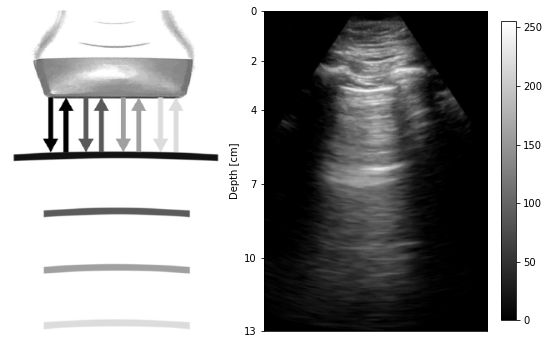
\includegraphics[width=\textwidth]{figuras/alines_plus.png}
		\caption{\footnotesize A-lines are the consequence of a reverberation artifact. Multiple back and forth reflections between the pleura and the transducer give rise to equally-spaced lines.}
		\end{subfigure}
		\centering
		\hspace{2em}
		\begin{subfigure}[b]{0.32\textwidth}
		\centering
		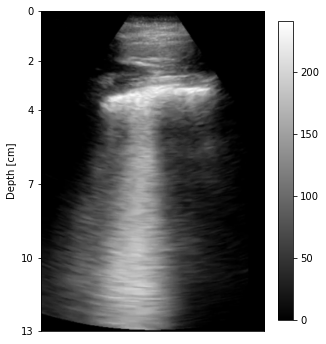
\includegraphics[width=\textwidth]{figuras/blines.png}
		\caption{\footnotesize B-lines are vertical artifacts originated by reverberation within the lung.}
		\end{subfigure}	
	\caption{\small A-lines (a) and B-lines (b) are common artifacts observed in lung ultrasound.}
	\label{artifacts}
	\end{figure}	


\section{Objectives}

	The present work explores lung ultrasound imaging (LUS) from different perspectives and with different goals.

	Firstly, it focuses on understanding ultrasound imaging from a theoretical point of view. It aims to identify the physical principles that rule its operation, as well as explaining the image artifacts that are characteristic of this technique. In particular, those artifacts present in lung ultrasound are explored.
	
	Secondly, the current state of research on LUS is explored in the scientific literature. Besides considering the broader context of medical physics to which the topic belongs to, emphasis is placed on recent applications of artificial intelligence to lung ultrasound.

	Lastly, a practical approach has also been taken on LUS in order to become familiarised with a programming language and other tools. An analysis of a collection of lung ultrasound videos has been carried out, and its results have been interpreted. The goal has been to design a machine learning model capable of detecting B-lines after being trained on a set of labelled images. This has been done taking two different approaches: first, by extracting those features of the image that are more likely to be correlated with B-line appearance; then, by feeding all the information in the images to the model.
	
	Apart from that, this work also mentions the results of a collaboration with the ULTRACOV project, with the aim to have a first experience in research.
	
	
% MÉTODOS
\section{Methods}

\subsection{Software tools}
	Different tools have been used throughout this work. Python programming language has been chosen to perform the analysis on the ultrasound videos due to its popularity among the scientific community and the wide offer of libraries available. These are collections of pre-written and documented code designed for different purposes: NumPy\cite{numpy} for matrix and numerical calculations, Matplotlib\cite{matplotlib} for graphs and visualizations, OpenCV\cite{opencv} for image analysis and Scikit-learn\cite{sklearn} for machine learning algorithms, among others.

	Appart from all the necessary libraries to develope our algorithms, an application to edit our code, test it and debug it is also needed: this is the role of an integrated development environment (IDE). Both Sypder\cite{spyder} and PyCharm\cite{pycharm} have been used.
	
	Finally, it is also useful to have some way of organising our code and handling updates. To this purpose, version control applications such as GitHub are of great help. They allow developers to save their source code online and keep track of any changes or updates. It is specially useful when collaborating with other developers.


\subsection{Data set}

	In this work we have made use of a collection of 240 ultrasound videos of lungs. The videos correspond to a single patient throughout a 40 day period of regular examinations monitoring the evolution of Covid-19 pneumonia. They were taken and labelled according to B-lines presence by an experienced physician (Dr. Yale Tung Chen \cite{tung2020lung}
	 - Hospital Universitario Puerta de Hierro) as part of the ULTRACOV project. All videos were taken with a Butterfly iQ probe set to 13 cm of scan depth. Most of the videos correspond to regions of the chest where the lung is the only visible organ, but on some of them other organs such as the liver or the spleen appear. An image resolution of 1080$\times$632 pixels and framerate of 21 fps is constant across the whole database. Video durations vary widely, ranging from 1 second to 20 seconds of length, with an average of 6 seconds per video. 
	
	Each video was labelled depending on whether B-lines were present or not at any instant throughout the video. In other words, videos labelled as 'no B-lines' do not exhibit them on any of their frames whereas videos labelled as 'B-lines' do, at least on a fraction of their frames but not necessarily in all of them. This is due to the natural motion of the lungs while breathing, as well as motion of the probe and changes in direction of observation. Because of this, it is necessary to  separate videos in smaller sections and isolate those corresponding to B-lines presence. A total number of 85 videos out of 240 are labelled as 'B-lines', which adds up to a $35 \%$ frequency of occurrence. 
	
	The frames of every video were extracted and cropped to remove unnecessary details for the later analysis. As a result, a collection of gray-scaled images sized 905$\times$632 pixels and 8 bits of depth (i.e., brightness values ranging from 0 to 255) was obtained. 
	
	\begin{figure}
	\centering
	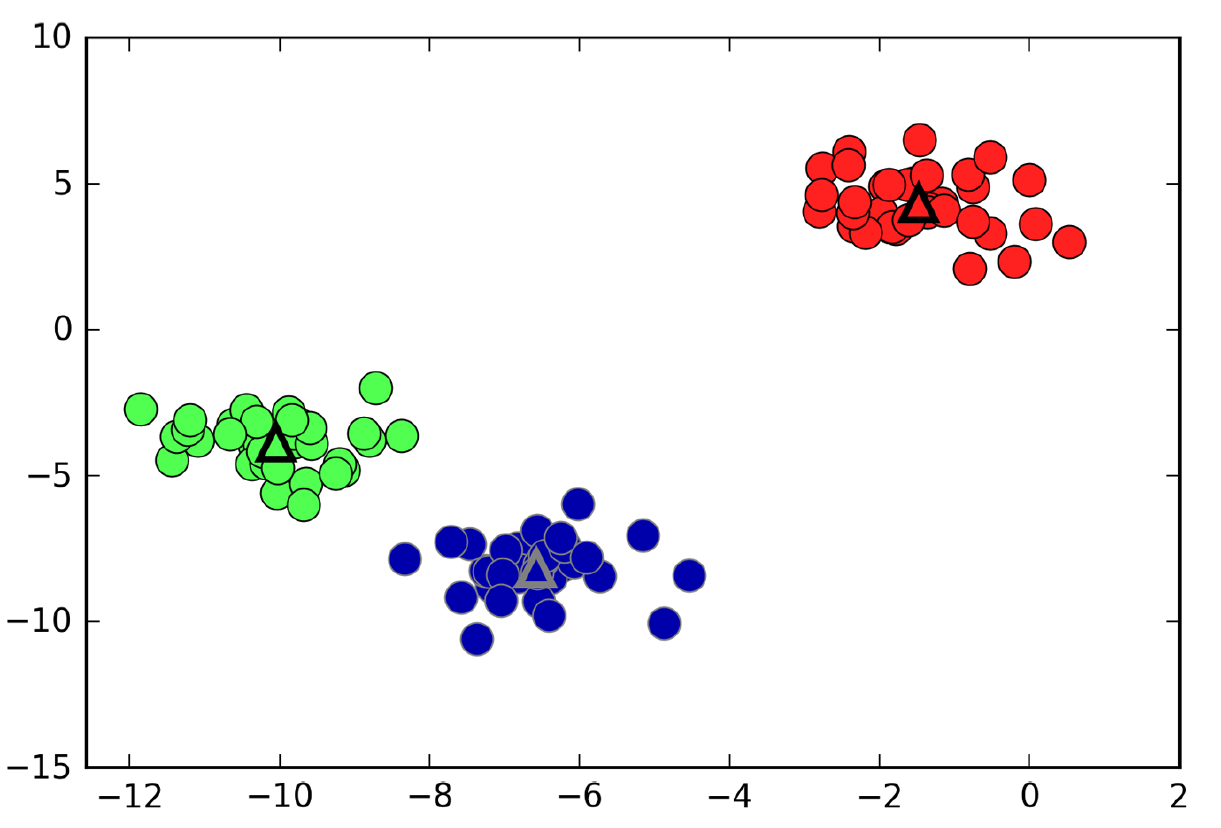
\includegraphics[width=8cm]{figuras/clusters.png}
	\caption{\small Representation of a K-Means algorithm for a two-dimensional data set. Each cluster (red, green, blue) is represented by its average or 'centroid' (triangles). Data points are assigned to the cluster whose centroid is the closest. The algorithm looks for the configuration whose 'inertia' or 'within cluster sum of squares' is minimised.\cite{python}}
	\label{clustering}
	\end{figure}
	
	In order to facilitate analysis it is useful to transform the original set of videos into a set of images. To achieve this, a K-means clustering algorithm implemented in the Scikit-learn toolkit was used \cite{sklearn}. Clustering algorithms are a kind of unsupervised learning algorithms whose aim is to subdivide a dataset into separate groups or clusters in such a way that data points belonging to the same cluster are as close as possible to each other. K-means is one of the simplest of these algorithms. When applied to a two-dimensional data set the result looks like shown in figure \ref{clustering}\cite{python}. Each cluster is represented by a cluster center or 'centroid', which corresponds to the average of the data points belonging to that cluster. Each data point is assigned to the cluster whose centroid is the closest. Different configurations are computed one after another until the total sum of distances within clusters is minimised, also known as 'inertia' parameter:
	
\begin{equation}
I = \sum_j^N \sum_{x_i \in C_j} || \vec{x_i} - \vec{ \mu_j} ||^2
\end{equation}
	
	where $N$ is the total number of clusters, $\vec{\mu_j}$ is the 'centroid' of the j-th cluster $C_j$ and $\vec{x_i}$ are data points.
	
	When working with images, instead of two dimensions each data point $\vec{x_i}$ belongs to an n-dimensional space with n being equal to the number of pixels in the image ($905 \times 632=571960$ in our case). For every video in the original collection  three clusters have been calculated and the closest frame to each cluster centroid was selected. On those videos labelled as 'B-lines' only the frames that do show B-lines have been manually selected. As a result, a set of $638$ labelled images was obtained, $173$ of which correspond to B-lines and the remaining $465$ showing no B-lines ($27 \% $ positives). An example of selected frames for a video through this method can be seen in figure \ref{key_frames}.
	

		
	\begin{figure}
	\centering
		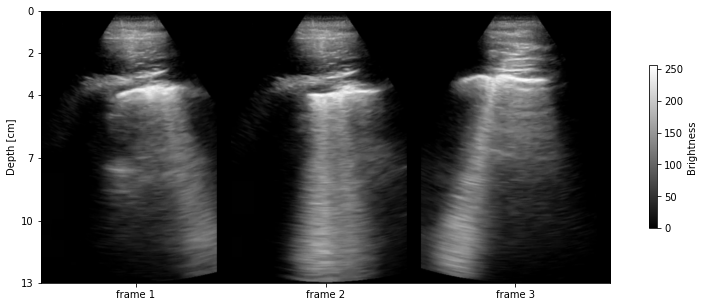
\includegraphics[width=\textwidth]{figuras/key_frames.png}
	\caption{\small Selected frames representing a video. A K-Means clustering algorithm was used to split every video into three clusters. The nearest frame to each cluster centroid was selected.}
	\label{key_frames}
	\end{figure}		
	
	

%	\begin{figure}
%	\centering
%		\begin{subfigure}{0.3\textwidth}
%		\centering
%		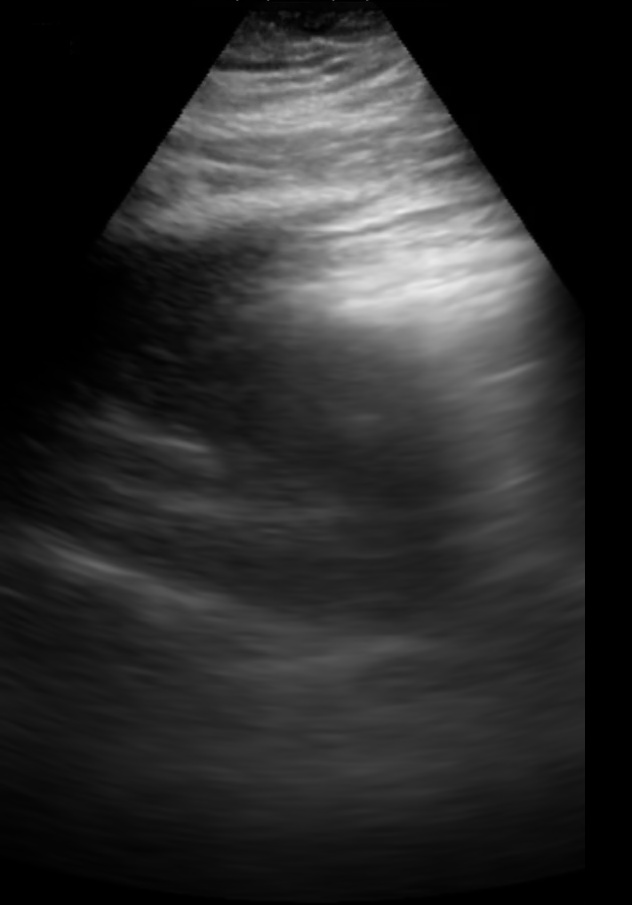
\includegraphics[width=\textwidth]{figuras/centroid_0.jpg}
%		\end{subfigure}
%		\begin{subfigure}{0.3\textwidth}
%		\centering
%		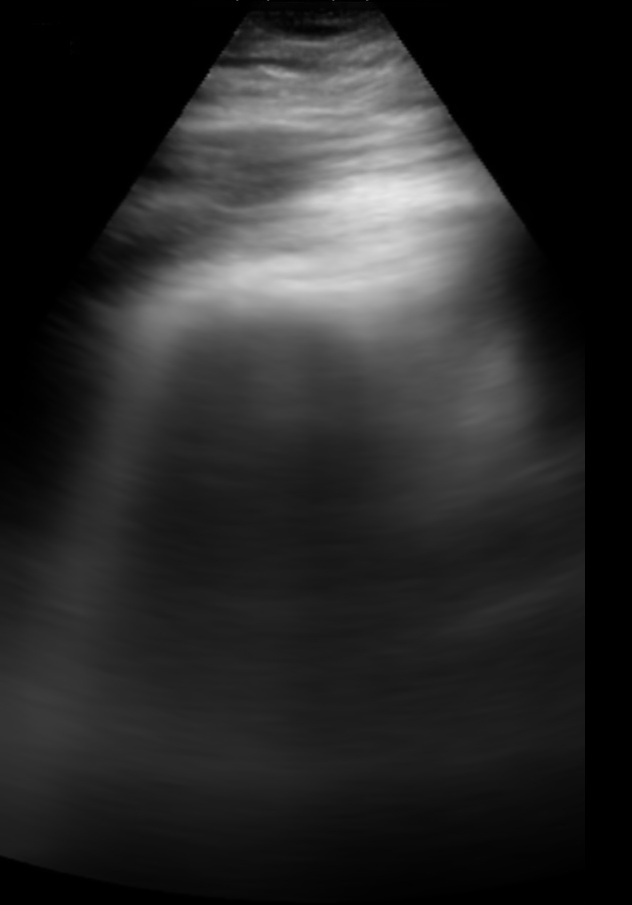
\includegraphics[width=\textwidth]{figuras/centroid_1.jpg}
%		\end{subfigure}
%		\begin{subfigure}{0.3\textwidth}
%		\centering
%		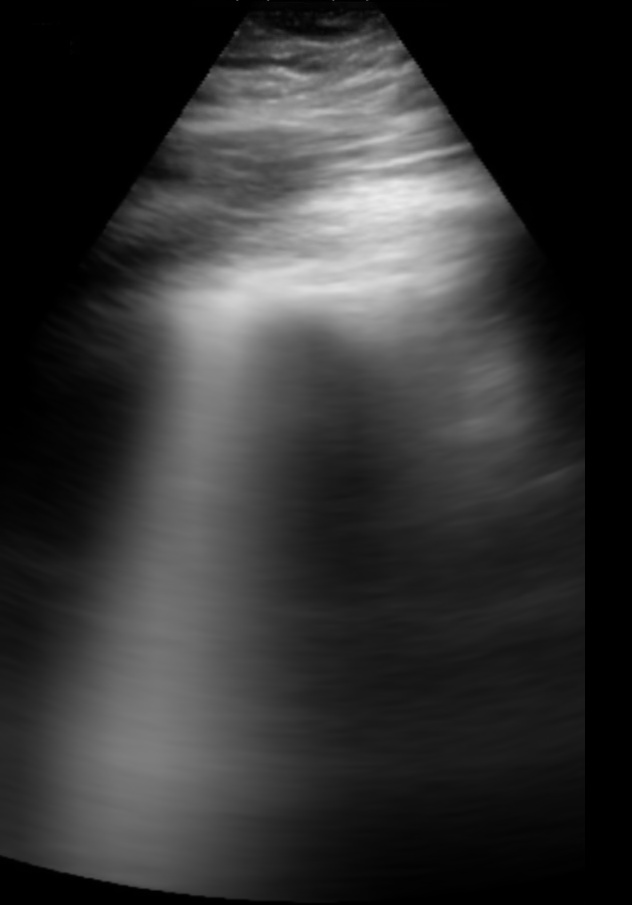
\includegraphics[width=\textwidth]{figuras/centroid_2.jpg}
%		\end{subfigure}
%	\caption{A set of three cluster centroids representing a single video}
%	\end{figure}

\subsection{Feature-based classification}
A classification of the image data set was first carried out with a feature-based approach. Images are assigned a score based on the analysis of certain characteristics typical of B-lines. An algorithm is then trained to classify images based on their scores.

\subsubsection{Polar format of ultrasound images}

	Before performing an analysis on the images it is useful to transform them into a more suitable format. A change of coordinates is performed on the ultrasound images in order to obtain images in a 'polar format' equivalent to what the raw data obtained by the ultrasound device would look like. In this format, vertical lines correspond to the signals received by the transducers. 
	
	To perform this change of coordinates, the aperture angle of the image is manually measured first. Next, the orignal 'sector format' image is split into regions of N equally-spaced radial coordinates and M angular coordinates. Finally, the mean brightness value of each region is calculated and assigned to the each pixel of the polar format image. By doing so, we obtained a rectangular-shaped image of N-rows by M-columns. In particular, we have chosen $N = M = 50$ (see fig.\ref{polar}). 
	
	This reshaping of the images facilitates further calculations for two reasons. Firstly, it speeds up calculations as we have greatly reduced the size of the images. Secondly, it also helps identify B-lines more easily, as they should now appear as vertical lines whereas originally they could be diagonal. 
	
%	\begin{figure}
%	\centering
%		\begin{subfigure}{0.29\textwidth}
%%		\centering
%		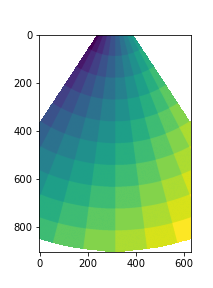
\includegraphics[width=\textwidth]{figuras/polar_original.png}
%		\caption{Sector-shaped image}
%		\end{subfigure}
%%		\hfill
%		\begin{subfigure}{0.35\textwidth}
%%		\centering
%		
\includegraphics[width=\textwidth]{figuras/polar_new.png}
%		\caption{Square-shaped image}
%		\end{subfigure}
%%		\hfill
%		\begin{subfigure}{0.30\textwidth}
%%		\centering
%		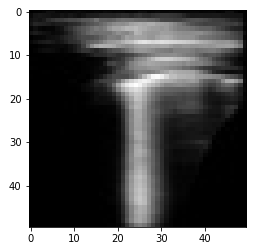
\includegraphics[width=\textwidth]{figuras/polar.png}
%		\caption{B-lines appear like vertical lines on this format}
%		\end{subfigure}
%	\caption{Reshaping of images into polar coordinates}
%	\end{figure}	
	
	
	\begin{figure}
	\centering
	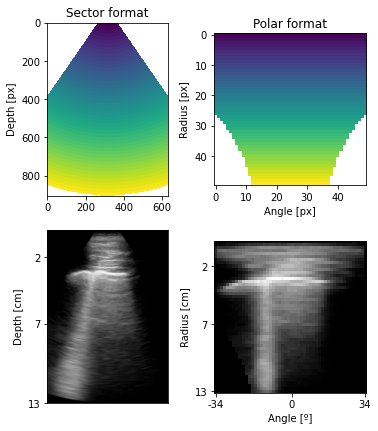
\includegraphics[width=0.5\textwidth]{figuras/sector_polar.png}
	\caption{\small Reshaping from sector format (left) into polar format (right). Radial and angular coordinates are subdivided into $N=M=50$ sections. Each region's mean brightness value is assigned to a pixel in a $N\times M$ rectangular image. As a result, rows represent equal radial coordinates and columns represent equal angular coordinates.}
	\label{polar}
	\end{figure}	
	
	
\subsubsection{Selected B-line features}

	A scoring system was then used to assess the likelihood of an image to contain B-lines. Such a scoring system must take into account known features of B-line pattern: bright, uniform vertical shapes extending from the pleural line to the lower margin of the image. Images exhibiting B-lines should generate high scores on this scale, whereas those who show none should produce lower scores. The score analysis is performed on the images in polar format. On this work five features have been taken into account:
	
\begin{itemize}
	\item \textbf{Column mean brightness}: average brightness is calculated for every column on the image. The highest value obtained is chosen as the outcome. All averages are calculated excluding the region above the pleural line, which is estimated to be located at the peak of brightness in that column.
	
	\item \textbf{Bottom quarter mean brightness}: average brightness is calculated for every column on the quarter section that is further away from the transducer. This feature accounts for the fact that B-lines strecht down to the lowest margin of the image, while other artifacts fade away faster.
	
	\item \textbf{Bottom value}: brightness values at the lowest point are taken for every column. The maximum value among them is selected.
	
	\item \textbf{Center of mass}: vertical center of mass coordinates are calculated below the pleura for every column using pixel brightness as weights. The highest value (lowest center of mass) is selected. 
	
	\item\textbf{Length times mean}: for every column its length excluding the region above the pleura (above peak brightness coordinate) is multiplied by its mean brightness. The highest value among them is selected.
	
\end{itemize}

Once analysed, every image can be represented by a set of five values corresponding to each feature. Images' brightness was previously normalised so that every score is in the $(0,1)$ range. It is important to note that other features could be taken into consideration. The present ones have been chosen due to its simplicity and easy interpretation.



\subsection{Image-based classification}
An image-based approach is also taken on the classification of the data set. This time the algorithm is fed the images without any previous feature extraction. That means the input data has now as many features as pixels in the image, with the brightness of each pixel being the value of the feature. To speed up calculations, images have been resized to a square $200 \times 200$ shape, which results in a $40000$-element vector representing every image (see fig.\ref{diagrama}).

	\begin{figure}[h]
	\centering
	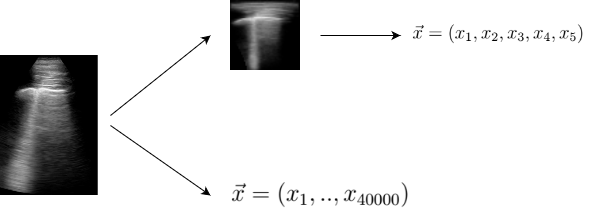
\includegraphics[width=11cm]{figuras/diagrama.png}
	\caption{\small Comparison of feature-based and image-based approaches. On the feature-based approach (upper part) images are represented by 5-element vectors. On the image-based approach (lower part) images are represented by 40000-element vectors.}
	\label{diagrama}
	\end{figure}
	
\subsection{Classification algorithm: logistic regression}
	Once the data has been properly transformed into a vector representation as previously described, it can be fed into the classification algorithm. This algorithm follows two phases. First, a traning phase where the model's parameters are adjusted to fit data. Then, a testing phase where the model's prediction is assessed. In order not to obtain a biased prediction, the data set and its accompanying labels (B-lines/no B-lines) must be randomly split into two subsets: a training set that is fed to the model in the training phase, and a testing set to be used in the testing phase. Ratios of 0.8 and 0.2 were chosen for the split between training and test set respectively. As a result, the model was trained on 510 data points and labels, and tested on the remaining 128 samples.

	Of all the classification algorithms available, a logistic regression algorithm has been chosen due to its simple working principle. Logistic regression is a kind of supervised learning algorithm that takes its name from the logistic or sigmoid function:
	
  \begin{equation}
    \sigma(t) = \frac{1}{1+ e^{-t}}
  \end{equation}	
  
  In this algorithm the logistic function takes the inner product of a data sample vector $\vec{x_i}$ and a weight vector $\vec{\theta}$ as an input to estimate the probability $p$ of that data sample belonging to one of two classes $y=0,1$:
  
\begin{equation}
p(\vec{x}, \vec{\theta}) = \sigma(\vec{x}\cdot\vec{\theta})
\end{equation}\break

	The predicted class $y$ is simply determined as the rounded probability $p$:


\begin{equation}
y =
\left\{
	\begin{array}{ll}
		0  & \mbox{if } p < 0.5 \\
		1 & \mbox{if } p \geq 0.5
	\end{array}
\right.
\end{equation}

	The weight vector $\vec{\theta}$ contains the free parameters that have to be adjusted during the training phase in order for the model to fit a given input set of data ${\vec{x_i}}$ and labels ${y_i}$. This is done with the help of a cost function $c(\vec{\theta})$ that quantifies how close the predicted probability of a data sample $p(\vec{x}, \vec{theta})$ is to its labelled class $y$:

\begin{equation}
c(\vec{\theta}) =
\left\{
	\begin{array}{ll}
		-\log{p}  & \mbox{if } y = 1 \\
		-\log{(1-p)} & \mbox{if } y = 0
	\end{array}
\right.
\end{equation}
	The cost function tends to infinity when the predicted class is opposed to the labelled class, and tends to zero when prediction and label match. Similarly, the average deviation between prediction and labels over a whole training set with $N$ samples is defined as the average value of the cost function $J(\vec{\theta})$:

\begin{equation}
J(\vec{\theta}) = -\frac{1}{N}\sum_{i=1}^{N} \left( y_i \log{p_i} + (1-y_i)\log{(1-p_i)} \right)
\end{equation}

The weight vector $\vec{\theta}$ that minimises this quantity is the one that best fits the training data.


\section{Results}

	Scores of all images in the training set have been calculated for every feature and its distributions have been represented in figure \ref{scores}. For each feature the score distributions for positive and negative B-line cases can be seen, and their mean values are indicated by vertical lines. Mean values for B-line cases are higher than those of non-B-line ones for each feature, which indicates that the selected features are indeed correlated with the presence or absence of B-lines on the images. However, there is some overlap between the values scored by positive and negative cases (i.e. presence or absence of B-lines). In other words, in this representation there is not a clear boundary between each class of data points. 
	
	
\begin{figure}[h]
\centering
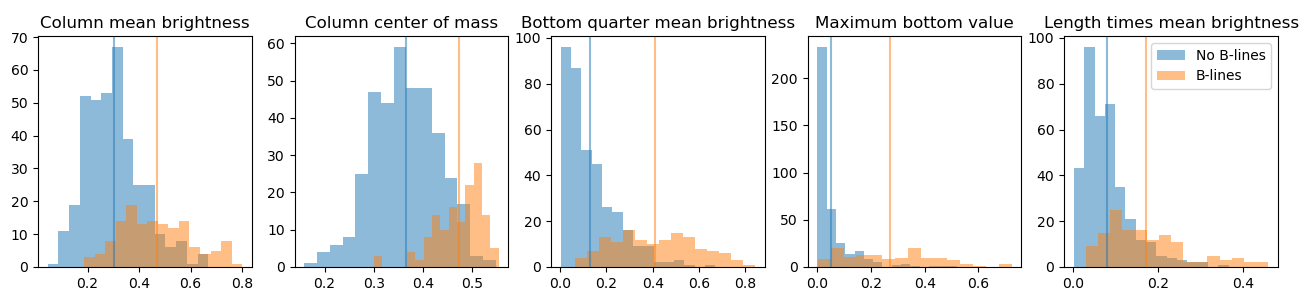
\includegraphics[width=\textwidth]{figuras/score_overview.png}
\caption{\small Score distribution of positive cases (orange, B-lines) and negative cases (blue, no B-lines) for every analysed feature. Although mean values (vertical lines) on different classes are distinct, there is also some overlap between classes' scores. An ideal feature would yield non-overlapping score distributions.}
\label{scores}
\end{figure}


	A comparison between the algorithm's prediction and the true values is summarized in figure \ref{confusion} for both methods in what is known as a 'confusion matrix'. Elements in the diagonal of the matrix are correct predictions (true positives or true negatives), while elements out of the diagonal are wrong predictions (false positives or false negatives). A series of statistical measures is used to assess how good the classification is. 
	
	
\begin{figure}
\centering
\begin{subfigure}{0.45\textwidth}
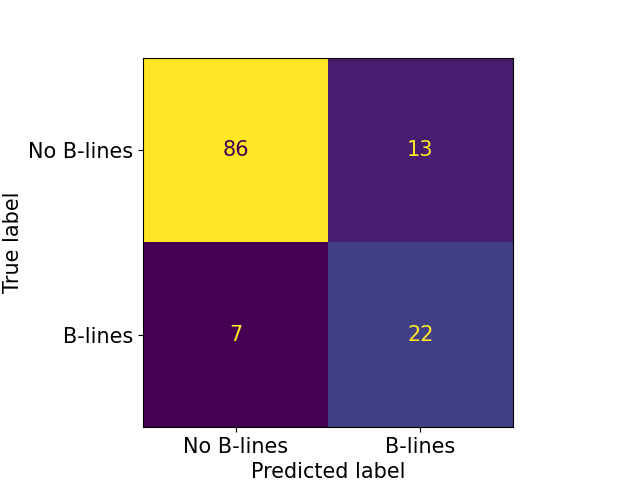
\includegraphics[width=\textwidth]{figuras/feature_confusion.png}
\caption{Feature-based classification}
\end{subfigure}
\begin{subfigure}{0.45\textwidth}
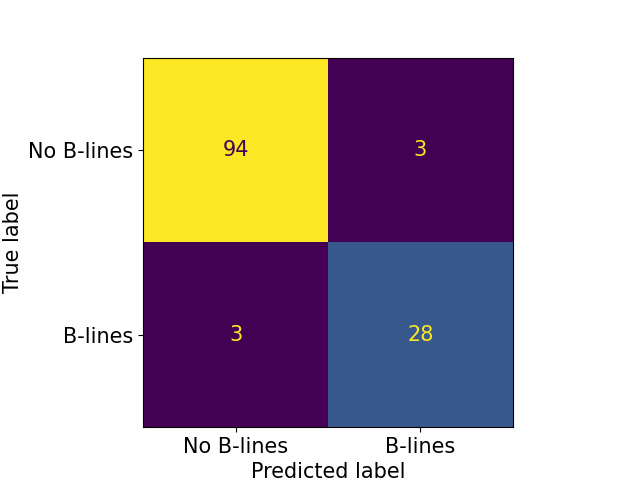
\includegraphics[width=\textwidth]{figuras/image_confusion.png}
\caption{Image-based classification}
\end{subfigure}
\caption{\small Confusion matrices of both approaches. Values correspond to number of samples out of 128 testing samples as follows (left to right, top to bottom): true negatives (TN), false positives (FP), false negatives (FN) and true positives (TP).}
\label{confusion}
\end{figure}	
	
	
	First, accuracy (ACC) is defined as the ratio of correct predictions (both true positives and true negatives) to the total number of cases: 
	
\begin{equation}
ACC = \frac{TP + TN}{TP + TN + FP + FN}
\end{equation}
	
	Sensitivity or 'true positive rate' (TPR) is defined as the ratio of correctly identified positives to the total number of real positives (true positives and false negatives):
	
\begin{equation}
TPR = \frac{TP}{TP + FN}
\end{equation}
	
	Conversely, specificity or 'true negative rate' (TNR) is the ratio of correctly identified negatives to the total number of real negatives (true negatives and false positives):
	
\begin{equation}
TNR = \frac{TN}{TN + FP}
\end{equation}
	
	Correct predictions can also be normalized against the number of predictions made for each class. In the case of positive predictions we have 'positive predictive value' (PPV), which is defined as the ratio of true positives to all predicted positives (true positives and false positives):
	
\begin{equation}
PPV = \frac{TP}{TP + FP}
\end{equation}
	
	 On the other hand, 'negative predictive vaue' (NPV) measures the ratio of true negatives to all predicted negatives (true negatives and false negatives):
	 
\begin{equation}
NPV = \frac{TN}{TN + FN}
\end{equation}
	
	Performance of both methods on all the previously mentioned statistical measures has been summarised in table \ref{results}.


\begin{table}[]
\resizebox{\textwidth}{!}{%
\begin{tabular}{@{}c|ccccc@{}}
\toprule
                  & \textbf{Accuracy} & \textbf{True positive rate} & \textbf{True negative rate} & \textbf{Positive predictive value} & \textbf{Negative predictive value} \\ \midrule
\textbf{Features} & 84,4\%            & 75,9\%                      & 86,9\%                      & 62,9\%                             & 92,5\%                             \\
\textbf{Images}      & 95,3\%            & 90,3\%                      & 96,9\%                      & 90,3\%                             & 96,9\%                             \\ \bottomrule
\end{tabular}%
}
\caption{\small Comparison of classification results: feature-based and image-based approaches. The image-based approach showed a better performance across every statistical measure.}
\label{results}
\end{table}


\section{Discussion}

	Of both methods, the image-based classification is the one that shows better results across all statistical measures. However, the feature-based method has some advantages, as it provides a better insight on what are the characteristics that make both classes distinguishable. 
	
	The poorer performance of the feature-based method can be explained by the score distribution of the data set. Due to the overlap in scores between images of different classes, the classifier algorithm cannot determine a clear boundary between classes.
	
	The reason behind the overlap of scores is in the scoring system itself, and it could be overcome by selecting more appropriate features. For example, the 'bottom quarter mean brightness' scale may not always be correlated with the presence of B-lines. When organs such as the spleen appear on a video, the brightness on the lower half of the image increases (see fig.\ref{spleen}) even if there are no B-lines. This could cause a false positive. There is also the case of images that do not show B-lines but have a high average brightness due uneven gain settings of the probe across the data set, thus inducing false positives as well.  Therefore, the performance of the feature-based method could be improved with more accurate features and more uniform data.
	
	
\begin{figure}[h]
\centering
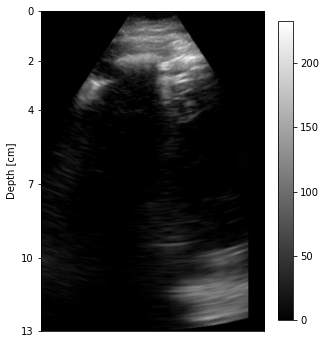
\includegraphics[width=0.4\textwidth]{figuras/spleen.png}
\caption{Potential false positives: presence of organs such as the spleen may be mistaken for B-lines with the current analysed features.}
\label{spleen}
\end{figure}
	
	
	A similar approach has been taken by Brattain et al. \cite{brattain}. In their study, pleural lines were removed from the images before evaluating the presence of B-lines, which might facilitate uniformity across the data set. Another approach by van Sloun \cite{vanSloun} used deep learning techniques, achieving accuracy of up to $90 \%$.

	
\section{Conclusion}
	Lung ultrasound (LUS) is a tool with great potential in healthcare due to its portability and safety of use. In combination with artificial intelligence techniques, it can provide a valuable and automated assessment of pneumonia-related lung diseases by detecting the presence of B-lines on the ultrasound imges. These are artifacts that can be understood as a consequence of the working principles of ultrasound imaging. A machine learning algorithm was trained on a labelled set of LUS images following two approaches. The image-based approach achieved a $95.3 \%$ accuracy, whereas the feature-based approach achieved $84,4 \%$ accuracy and could be improved. The proposed method could be also applied to the LUS data currently being gathered as part of the ULTRACOV project (see Appendix), which aims to develop an ultrasound scanner for the automated detection of COVID-19.

\section{Appendix}
\subsection{Source code}
Accompanying Python scripts can be found in the following GitHub repository:

{\textit{https://github.com/igortega/B-lines}}


\subsection{ULTRACOV project}
	The present work has taken place together with a collaboration with ULTRACOV project has also been made. ULTRACOV project \cite{ultracov} aims to develop an ultrasound device specific for Covid-19 detection. To this purpose, different AI algorithms are being developed. The device is currently undergoing clinical trials at Hospital Universitario Puerta de Hierro and Hospita Isabel Zendal.
	These analysis tools have also been gathered and integrated in a graphical user interface (GUI) using Python and the PySimpleGUI library (see fig.\ref{GUI}). The GUI also allows to display videos, manually assign labels to them based on the anomalies that they show and calculate a score of lung involvement. 
	
	The following tools have been included:
	\begin{itemize}
	\item Motion detection: it provides a graph of the lateral displacement in pixels of the video through an optical flow algorithm.
	\item Pleura detection: it shows the predicted location of the pleural line on the current video using a pre-trained neural network.
	\item Similar images: it displays a selection of the most similar images to the current one from a dataset.
	\item Image quality: it analyses whether the probe is properly placed based on the pleura detection tool (if no pleura can be seen the quality is not good).
	\end{itemize}
	
\begin{figure}[h]
\centering
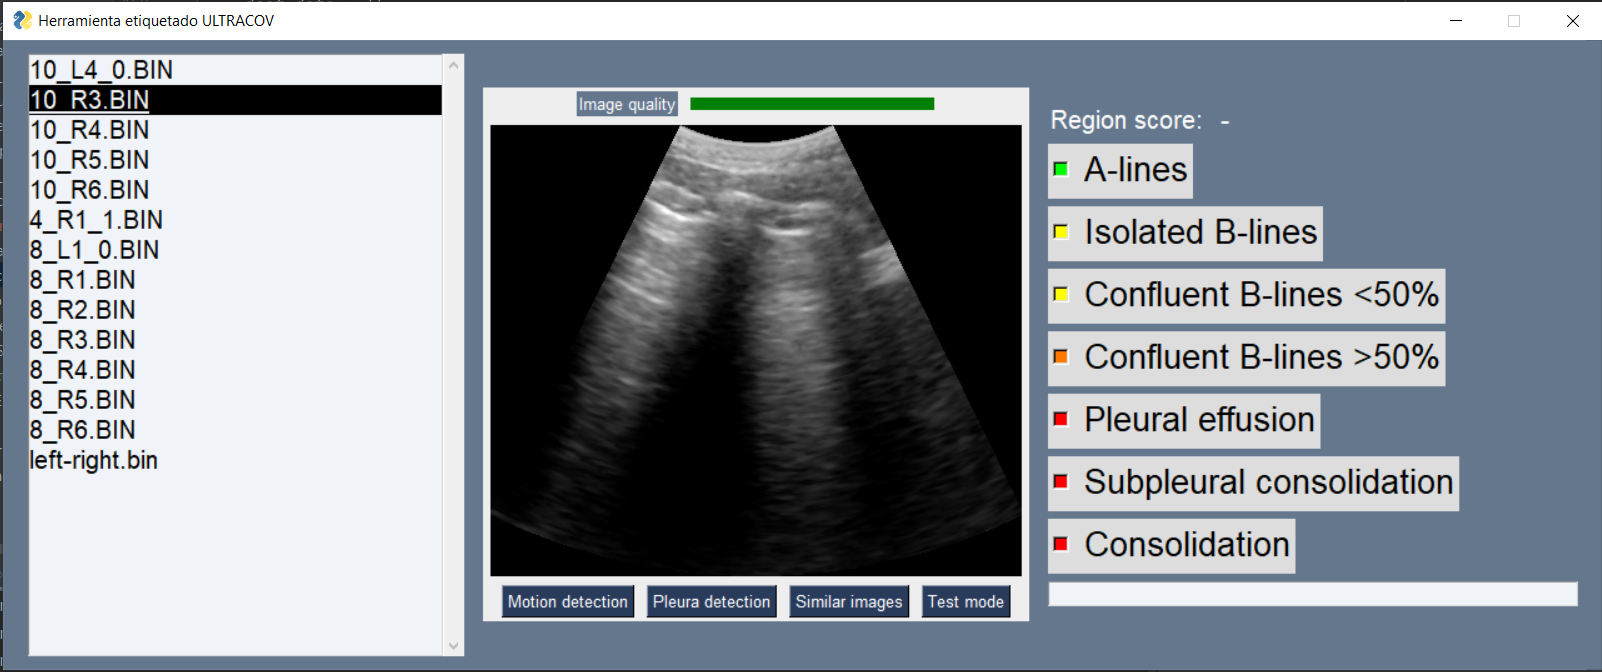
\includegraphics[width=0.9\textwidth]{figuras/ultracov_GUI.png}
\caption{\small Graphical user interface (GUI) including analysis tools for ULTRACOV project. Different tools are integrated in the GUI, such as a 'pleura detector' that automatically identifies the pleural line (in yellow on the image).}
\label{GUI}
\end{figure}

% BIBLIOGRAFÍA
\newpage
\newpage
\bibliography{biblio}
\bibliographystyle{plain}




\end{document}
